% !TEX root = acl_lualatex.tex
% HerHealthGPT-LU / LUHME 2026 — Introduction and Related Work
% Double-blind safe. Included from acl_lualatex.tex via \input.

    


\section{Introduction}
\label{sec:intro}
The central question in this work is not whether a large language model (LLM)
can produce a plausible answer to a women's-health question, but whether it
first understands what the user is trying to communicate.

\begin{figure*}
\centering
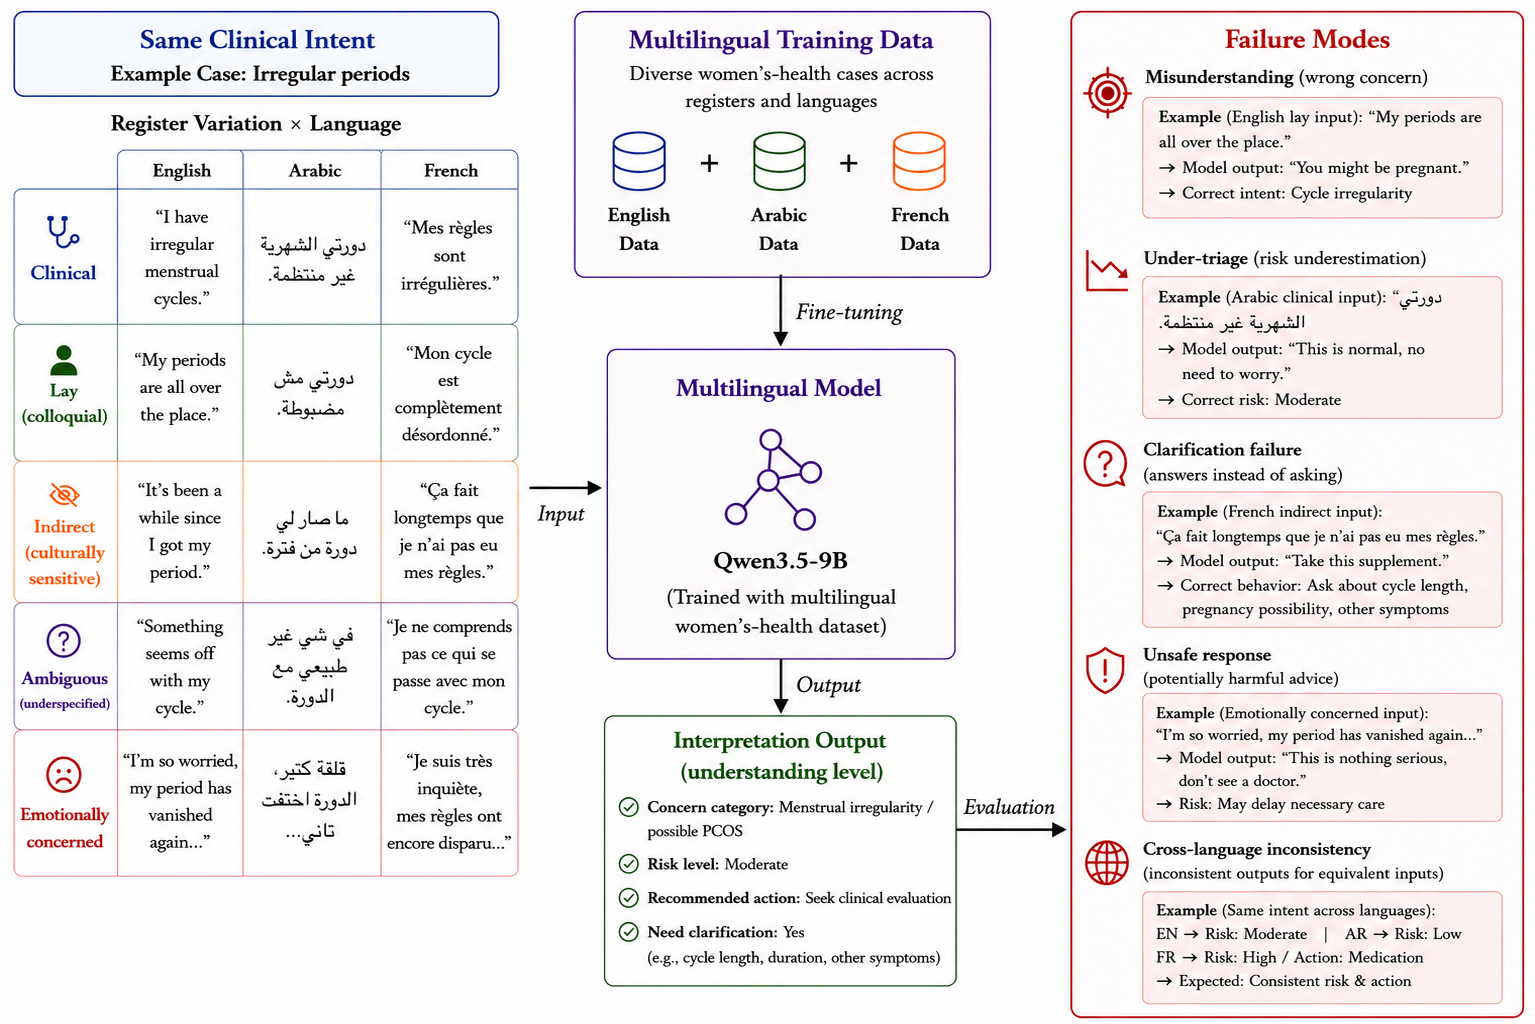
\includegraphics[width=0.8\textwidth]{figures/concept_overview.png}
\caption{\footnotesize Overview of the HerHealthEval evaluation framework.}
\label{fig:concept}
\end{figure*}
For example, the same irregular-menstruation concern may be expressed
clinically in French as
\foreignlanguage{french}{« Quelles sont les étiologies courantes des saignements
menstruels irréguliers ? »}
(``What are the common causes of irregular menstrual bleeding?''),
or more indirectly as
\foreignlanguage{french}{« Qu'est-ce qui pourrait expliquer un cycle menstruel qui change
sans cesse et n'est pas stable ? »}
(``What might explain a menstrual cycle that keeps changing and is not
stable?'').
In Modern Standard Arabic, the corresponding clinical formulation is
\foreignlanguage{arabic}{ما هي الأسباب الشائعة لنزيف الدورة الشهرية غير المنتظم؟}
(``What are the common causes of irregular menstrual bleeding?''),
whereas a more indirect formulation is
\foreignlanguage{arabic}{ما الذي قد يكون وراء دورة الحيض التي تتغير باستمرار وليست مستقرة؟}
(``What might be behind a menstrual cycle that keeps changing and is not
stable?''). These examples are drawn from the matched, validated variants in our evaluation suite. Although these expressions preserve the same underlying concern, they provide
different linguistic evidence to the model and may therefore trigger different interpretations and responses.

Misinterpreting such variation can cause a model to confuse the underlying concern, understate its urgency, offer false reassurance, recommend an inappropriate action, or respond directly when it should first request missing information \cite{recker-etal-2025-large,devries-etal-2025-enhancing}. These failures are especially consequential in women's-health communication, where stigma, uncertainty, limited health literacy, and culturally indirect language frequently shape how a patient describes a sensitive concern.

While existing studies of large language models in women's health primarily evaluate the quality of generated responses, they largely overlook whether the user's underlying concern was correctly understood. Furthermore, multilingual medical question-answering benchmarks have shown that identical clinical intents can elicit highly inconsistent recommendations across languages. Together, these limitations motivate a controlled evaluation of model interpretation rather than another answer-generation study. This paper presents \textbf{HerHealthEval} (See Fig.~\ref{fig:concept}), an evaluation framework for  language understanding in multilingual women's-health communication.
The evaluation suite spans menstruation, PCOS/hormonal concerns, and fertility, holding each underlying case fixed while varying canonical, clinical, layperson, indirect/culturally sensitive, ambiguous, and emotionally concerned expression.
Matched English cases are localized into Arabic and French under several native-speakers-approved protocol before entering cross-lingual evaluation or adaptation.
Each item has predefined targets for concern category, risk level, recommended action, and clarification need, and the evaluation lineage is kept separate from the adaptation corpus by source- and paraphrase-family exclusion.



We organize the study around three key research questions:
\begin{enumerate}
    \item \textbf{RQ1:}
    How robust are LLMs to variation in linguistic register when interpreting
    semantically equivalent women's-health concerns?
    \item \textbf{RQ2:}
    Do LLMs exhibit systematic differences in concern interpretation, triage
    calibration, recommended action, and clarification behavior across
    English, Arabic, and French?
    \item \textbf{RQ3:}
    How do English domain adaptation and joint English--Arabic--French
    adaptation affect linguistic robustness, uncertainty handling, and clarification behavior in women's-health communication?
\end{enumerate}


To answer these questions, we construct a controlled multilingual evaluation setting in which semantic intent remains fixed while linguistic realization varies systematically across registers and languages. Using HerHealthEval, we compare a general-purpose multilingual foundation model (Qwen3.5-9B-Instruct) with an English domain-adapted variant and a jointly adapted English--Arabic--French variant using the proposed HerHealthEval framework.


Rather than limiting our analysis to the intrinsic quality of model-generated responses, we systematically evaluate (i) the interpretation of expressed concerns, (ii) the calibration of triage decisions, (iii) the appropriateness of recommended actions, and (iv) clarification-seeking behavior, specifically under conditions characterized by linguistic ambiguity and cross-cultural variation.

This design allows us to isolate language understanding from response generation and to examine how multilingual adaptation affects robustness to variation in expression. 

Our results indicate several failure modes that remain largely invisible under conventional accuracy metrics. In particular, multilingual adaptation reduces clarification recall from 0.856 to nearly zero while increasing under-triage in French to 0.994 despite improving cross-language consistency. These findings suggest that apparent robustness under aggregate metrics may conceal substantial degradation in uncertainty handling and patient safety.

The remainder of this paper is organized as follows.
Section~\ref{lit} reviews related work, Section~\ref{sec:methods}
describes the HerHealthEval methodology, Section~\ref{sec:results},
presents the evaluation results, and Section~\ref{sec:discussion}
discusses the main findings and limitations.

\section{Literature Review}
\label{lit}

\begin{table*}[t]
\centering
\small
\begin{tabular}{p{0.16\textwidth}p{0.20\textwidth}p{0.14\textwidth}p{0.18\textwidth}p{0.20\textwidth}}
\hline
\textbf{Study} & \textbf{Goal} & \textbf{Languages Covered} & \textbf{Matched semantic variants} & \textbf{Explicit triage / clarification targets} \\
\hline
MenstLLaMA \citep{adhikary-etal-2025-menstrual} & Educational answer generation & English & No & No \\
Mai \citep{mughal-etal-2025-mai} & Menstrual-health dialogue generation & English, Roman Urdu & No & No \\
WHBench \citep{maurya-etal-2026-whbench} & Expert-scored clinical responses & English & No & Safety rubric; no clarification target \\
\textbf{HerHealthEval (proposed)} & Symptom-language understanding & English, French, Arabic adaptation data) & Yes & Yes \\
\hline
\end{tabular}
\caption{Positioning against the closest women's-health LLM systems. French and Arabic here refer to the adaptation-data languages; the scored evaluation set is English (\ref{sec:limitations}).}
\label{tab:positioning}
\end{table*}

This section reviews prior work on women's-health LLM evaluation,
multilingual and sociocultural language understanding, and
clarification-centered dialogue evaluation.
\subsection{Women's-Health LLM Evaluation}

Recent work has increasingly explored the use of LLMs for women's-health communication, primarily evaluating the quality of generated responses in terms of factuality, readability, empathy, and safety \citep{recker-etal-2025-large,devries-etal-2025-enhancing}.

Domain-adapted systems such as MenstLLaMA \citep{adhikary-etal-2025-menstrual} and Mai \citep{mughal-etal-2025-mai} demonstrate the potential of adaptation for menstrual-health dialogue, while PCOS and fertility studies largely evaluate clinician-authored questions or expert judgments of generated responses \citep{devranoglu-etal-2024-chatgpt,graca-etal-2026-assessing,chervenak-etal-2023-promise,gely-etal-2026-large}. WHBench further broadens coverage through expert-designed safety rubrics and structured response evaluation \citep{maurya-etal-2026-whbench}.

%Despite their differences, these studies share a common assumption: the input concern is already correctly understood. Consequently, they evaluate response generation rather than the interpretation process that precedes it.

%Together, these findings suggest that evaluating multilingual healthcare systems requires controlling semantic intent while varying linguistic realization across languages and cultures.



\subsection{Multilingual and Sociocultural Language Understanding}

Multilingual healthcare evaluation has shown that semantically equivalent
questions can elicit substantially different recommendations across
languages.
XLingEval evaluates correctness, consistency, and verifiability across
English, Spanish, Chinese, and Hindi, revealing considerable cross-language
variation in medical responses
\citep{jin-etal-2024-better}.
Subsequent studies similarly report inconsistent advice for equivalent
clinical questions across languages
\citep{schlicht-etal-2025-consistent}.

More broadly, cross-cultural NLP distinguishes linguistic variation from
cultural variation, identifying language form, shared knowledge, topic
relevance, and communicative goals as distinct dimensions of understanding
\citep{hershcovich-etal-2022-challenges,
adilazuarda-etal-2024-towards}.

In reproductive health, participatory studies show that culturally
appropriate responses often require local context beyond literal translation
\citep{deva-etal-2025-family}, while Western-centric evaluation rubrics may
systematically underrate culturally appropriate responses
\citep{dey-etal-2025-beyond}.

Recent LUHME work identifies related problems:
models compress cultural variation
\citep{mohammadi-etal-2025-large},
adaptation can fail when sociocultural context is ignored
\citep{freitas-cardoso-2025-nightmare},
and dialogue systems require mechanisms for establishing common ground
\citep{anikina-etal-2025-building}.


\subsection{Ambiguity, Clarification, and Understanding-Centered Evaluation}

Clarification research treats recognizing uncertainty, identifying missing
information, requesting additional evidence, and responding after
clarification as distinct capabilities that remain challenging for current
dialogue systems
\citep{testoni-fernandez-2024-asking,
zhang-choi-2025-clarify}. Structured and stateful dialogue systems that progressively elicit missing
information have therefore emerged as one practical direction
\citep{demarco-etal-2024-converso}

\subsection{Gap and Evaluation Requirements}
The resulting gap is therefore not another response benchmark, but an evaluation framework that measures whether models preserve the same underlying concern when equivalent meanings are communicated through different registers, languages, and sociocultural contexts.

Table~\ref{tab:positioning} summarizes the closest women's-health LLM systems and illustrates this gap. Existing systems primarily evaluate educational response generation, expert-scored answer quality, or dialogue helpfulness, while HerHealthEval focuses on multilingual symptom-language understanding through matched semantic variants and explicit triage and clarification targets.

Such an understanding-centered evaluation framework requires four properties:


\begin{enumerate}
    \item preserving semantic intent while varying linguistic realization
    across registers and languages;
    
    \item evaluating concern interpretation, risk assessment, recommended
    actions, and clarification behavior separately;
    
    \item exposing under-triage and unsafe recommendations rather than
    relying solely on aggregate accuracy; and
    
    \item preventing contamination between adaptation and evaluation data.
\end{enumerate}

HerHealthEval, operationalizes these requirements through matched multilingual
register variants, explicit interpretation targets, and a leakage-control
protocol based on source and paraphrase-family exclusion.

